\section{Experimental Evaluation}\label{sec:exp}

\subsection{Experiment Settings}

We evaluate the proposed technique over the FourSquare check-in dataset~\cite{yang2014modeling}. The dataset contains 227,428 check-ins in New York city and 573,703 check-ins in Tokyo collected in a duration of 10 month. We are interested in the user ID, PoI ID, check-in time stamp, and the PoI category of each record. We use the user rating of PoIs on FourSquare as ground truth. Specifically, FourSquare uses a 10-points based rating system. A high score indicates a good rating. The score is computed based on user's selection of three options: ``Like" (10 points), ``Neither like nor dislike" (5 points), or ``Dislike" (0 point). For comparison purpose, we have implemented three schemes:
\begin{itemize}
\item{Linear regression (LR)} A baseline approach that predicts user ratings with a model generated by simple linear regression with the proposed features.
\item{Matrix factorization (MF)} The simple non-negative matrix factorization~\cite{koren2009matrix} for recommender systems. We use matrix factorization to predict the rating of each users who have visited a PoI, then use their average rating score as the predicted rating of the PoI.
\item{Deep neural network (DNN)} The scheme predicts user ratings with a model trained by deep neural network as proposed in Section~\ref{sec:prediction}, using the proposed features as input.
\end{itemize}

Key parameters of our experiment is given in Table~\ref{settings}. For LR and DNN, we use the four types of features discussed in Section~\ref{sec:method}. As for MF, it does not rely on any explicit feature. Our experiment platform is a virtual machine with Intel Xeon 64-bit 8-core CPU running on 2.93GHz and 32GB RAM. The algorithms are implemented with Microsoft Azure machine learning toolkit and modules. 

\begin{table}[htbp]
\begin{center}
\caption{Groups based on how often user visits a location \label{settings}}
\begin{tabular}{|l|c|} \hline
\textbf{Parameter} & \textbf{Default value} \\ \hline
Number of users & 5000  \\ \hline
Number of PoIs & 1500 \\ \hline
Training set size (\%) & 10\% \\ \hline
Neural network depth (for DNN)& 3 \\ \hline
Number of latent features (for MF) & 8 \\ \hline
\end{tabular}
\end{center}
\end{table}

\subsection{Data Cleaning}

A few data cleaning steps are needed to prepare the dataset. First, we remove the PoIs which do not have user rating or were rated by less then 20 users. Second, we also remove the \textit{inactive} users from the dataset. We define inactive users as those who have less than 2 check-ins per week in the 10 month period. The lack of data makes it hard to extra the aforementioned features based on these user's trajectory. After the cleaning process, we extract the check-in information of approximately 5000 most active users and 1500 PoIs they have visited from the dataset.

In order for MF to work, we generate a user-PoI rating matrix based on the users and PoIs appeared in the FourSquare dataset. The user ratings are directly crawled from FourSquare. It is possible because which PoI is liked or saved by a user is publicly available.

\subsection{Prediction Results}

\begin{figure}[htbp]%
        \centering
        \begin{subfigure}{0.25\textwidth}
               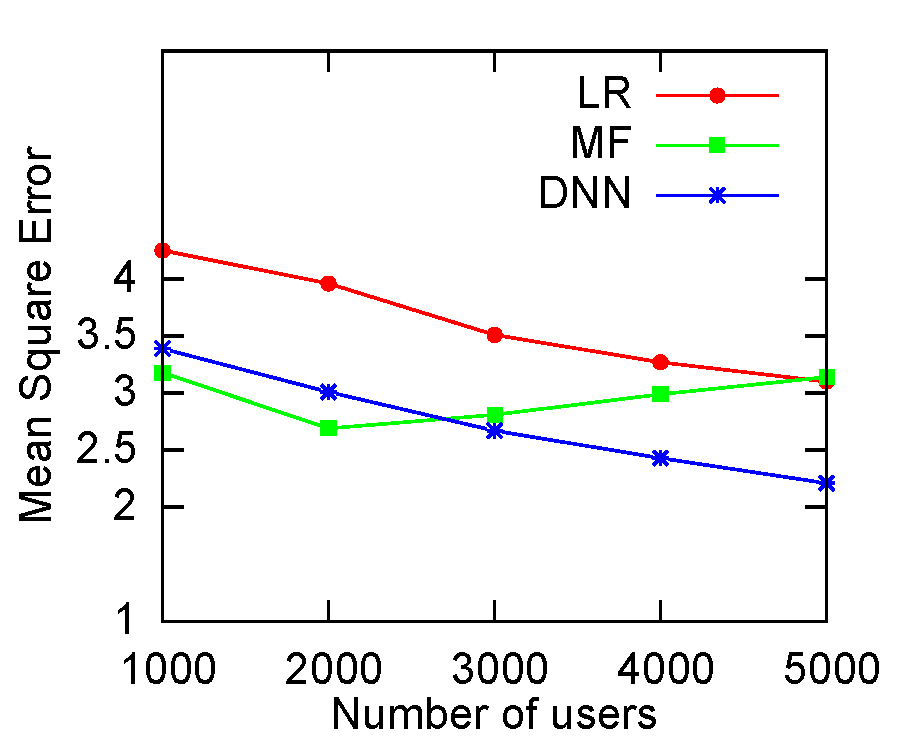
\includegraphics[scale=0.25]{E1.pdf}
        \end{subfigure}%
        ~ %add desired spacing between images, e. g. ~, \quad, \qquad, \hfill etc.
          %(or a blank line to force the subfigure onto a new line)
        \begin{subfigure}{0.25\textwidth}
                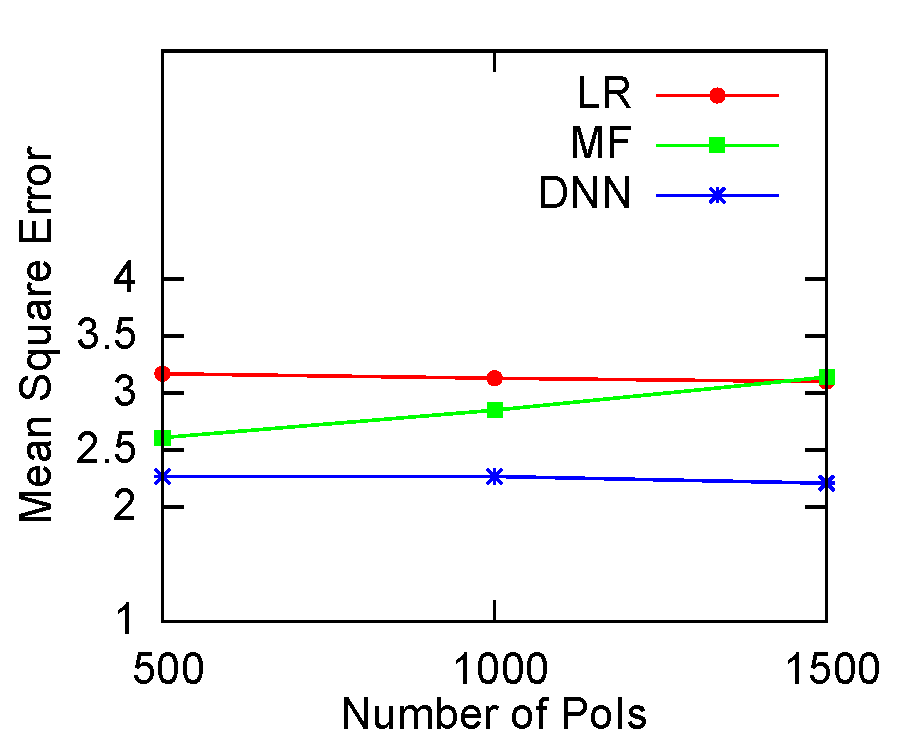
\includegraphics[scale=0.25]{E2.pdf}
        \end{subfigure}
         \caption{MSE of different prediction schemes}\label{E12}
         \vspace{-2mm}
\end{figure}

We first compare the Mean Square Error (MSE) of the prediction results of the three schemes. For each test point, we use a different number of number of users and PoIs, respectively, and exam the trend of performance of the compared schemes. The result is plotted in Figure~\ref{E12}. The proposed DNN prediction method demonstrate clear advantage over the other two scheme given a moderate number of users. The performance of the baseline method is also close to that of pure matrix factorization for a larger number of users. The performance of DNN increases as the number of users increases. This implies a larger group of users demonstrates more reliable spatial-temporal features for rating prediction. In contrast, the performance of MF drops as the number of users/PoI increases. This is because as the size of user-PoI rating matrix increases, it becomes significantly more spares, making it harder for MF to generate accurate predicts. The number of PoIs used have relatively small impact on the proposed prediction method.

\begin{figure}[htbp]%
        \centering
        \begin{subfigure}{0.25\textwidth}
               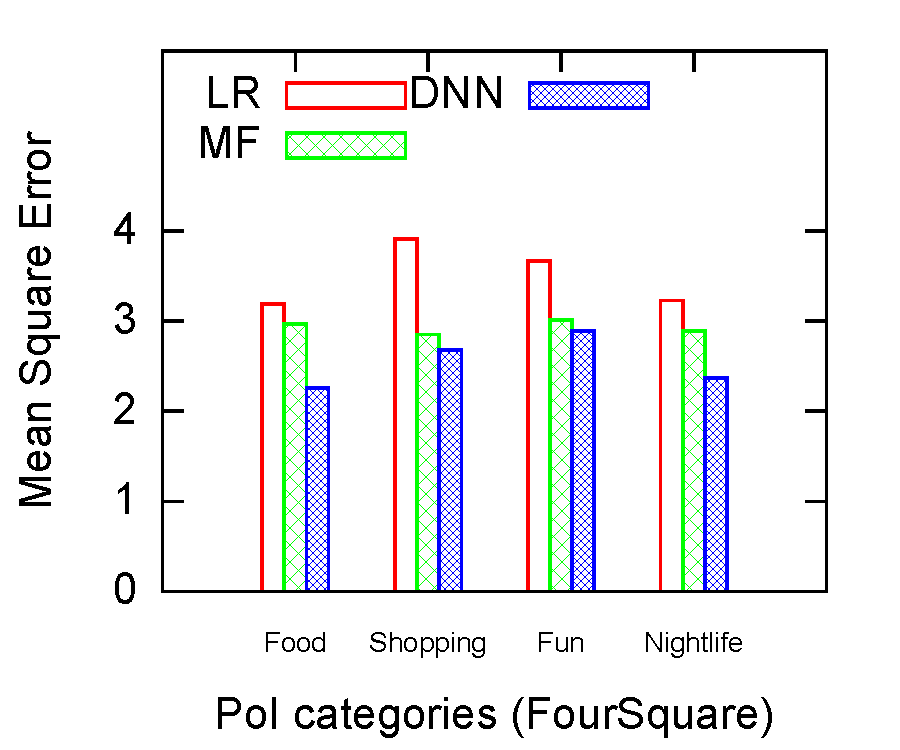
\includegraphics[scale=0.25]{E3-a.pdf}
        \end{subfigure}%
        ~ %add desired spacing between images, e. g. ~, \quad, \qquad, \hfill etc.
          %(or a blank line to force the subfigure onto a new line)
        \begin{subfigure}{0.25\textwidth}
                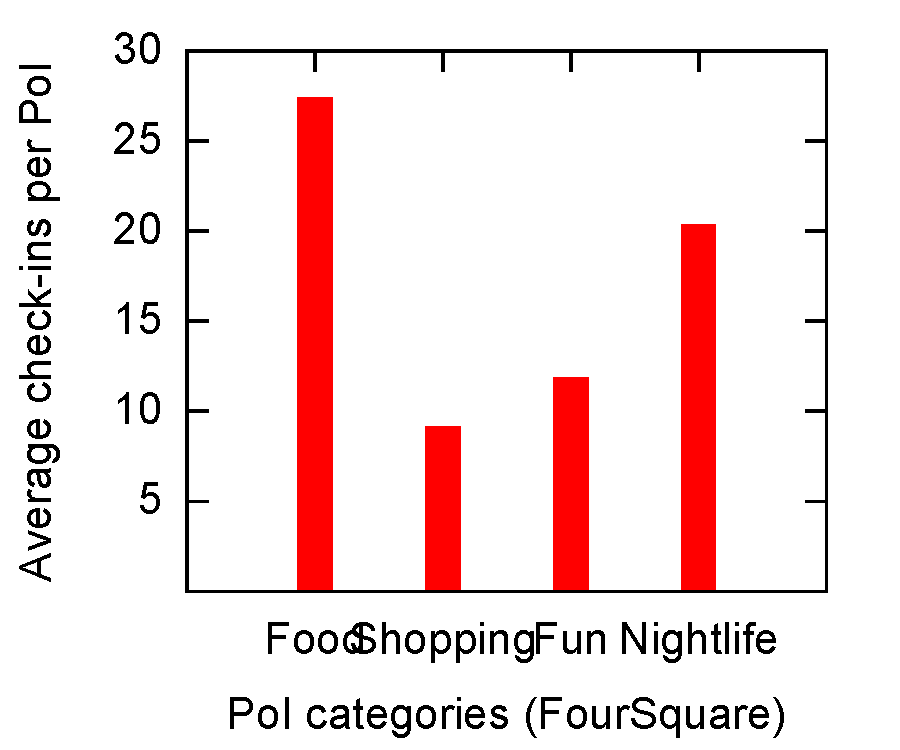
\includegraphics[scale=0.25]{E3-b.pdf}
        \end{subfigure}
         \caption{MSE of different PoI categories}\label{E3}
         \vspace{-2mm}
\end{figure}


We also shows the MSE of the prediction result for PoIs in four different categories, namely ``Food", ``Shopping", ``Fun", and ``Nightlife". These PoI categories are provided by FourSquare. There appears to be a difference of prediction accuracy between PoI categories (Figure~\ref{E3}-a). For the proposed methods, the prediction result for ``Food" and ``Nightlife" shows a lower MSE comparing with that of ``Shopping" and ``Fun". A closer look at check-in data in different PoI category reveals that users reported less check-ins for ``Shopping" and ``Fun" PoIs comparing with that of `Food" and ``Nightlife" (Figure~\ref{E3}-b). Thus the relatively worse performance can be explained by the lack of data, which may affect the quality of extracted features.

\begin{figure}[htbp]%
        \centering
        \begin{subfigure}{0.25\textwidth}
               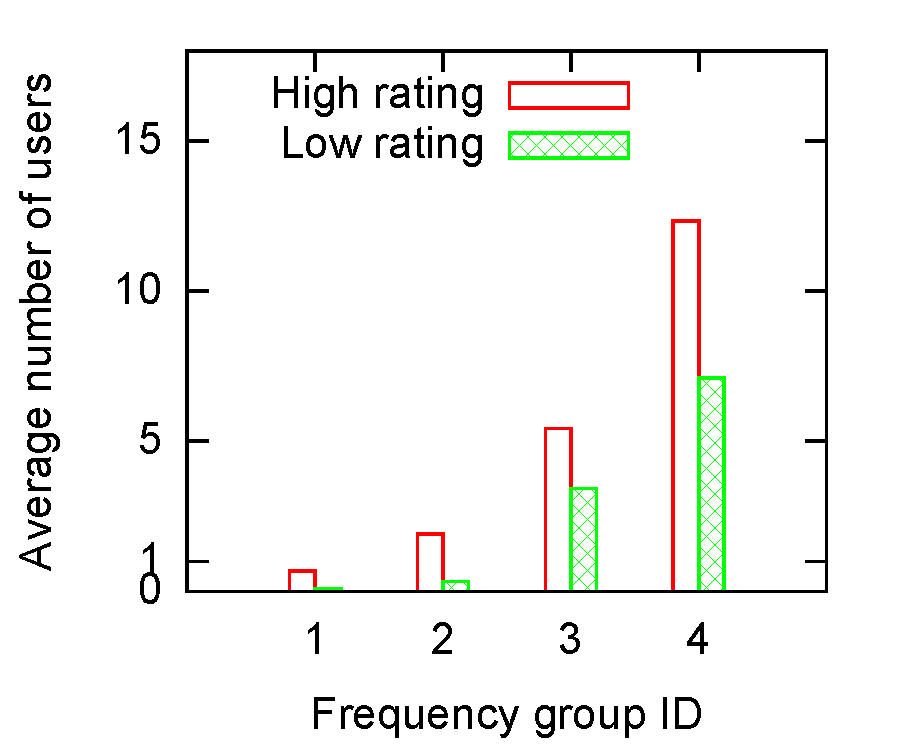
\includegraphics[scale=0.25]{E4-a.pdf}
        \end{subfigure}%
        ~ %add desired spacing between images, e. g. ~, \quad, \qquad, \hfill etc.
          %(or a blank line to force the subfigure onto a new line)
        \begin{subfigure}{0.25\textwidth}
                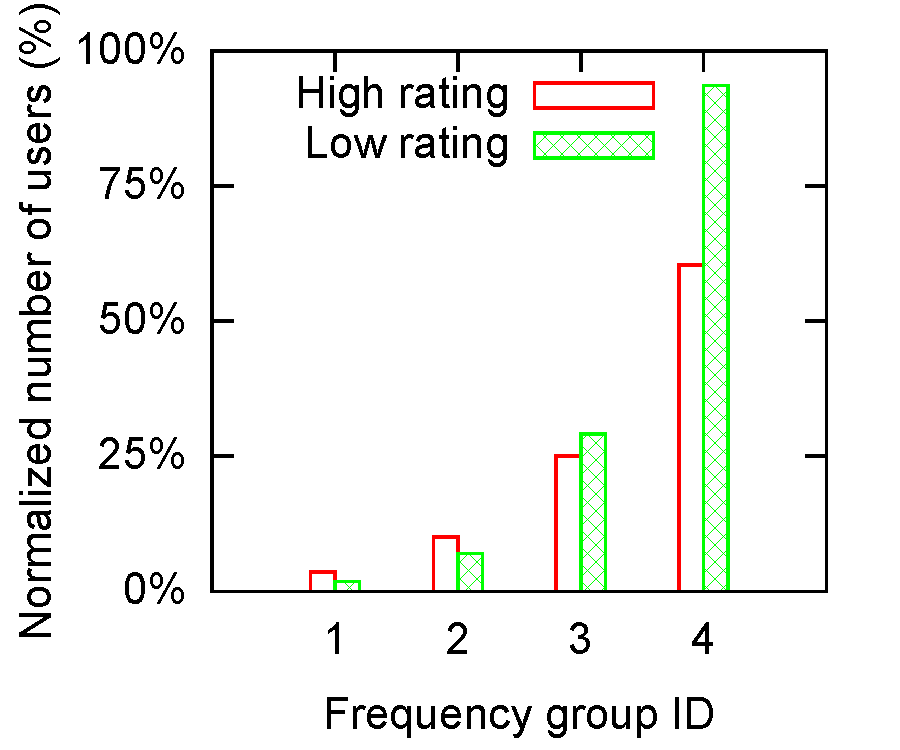
\includegraphics[scale=0.25]{E4-b.pdf}
        \end{subfigure}
         \caption{User frequency group distribution}\label{E4}
         \vspace{-2mm}
\end{figure}

Figure~\ref{E4} compares PoIs with different ratings in terms of the (normalized) average number of user in each frequency group, as showed in Table~\ref{frequencyGroups}. We observe that a highly rated PoI attracts more frequent-visitors comparing with PoIs with low ratings. This result supports the assumption we made in Section~\ref{sec:method}.
